\documentclass[10pt]{article}
\usepackage[a4paper, margin=2cm]{geometry}
%\usepackage{fullpage}
\usepackage[T1]{fontenc}
\usepackage[utf8]{inputenc}
\usepackage{graphicx}
\usepackage{mathpazo}
\pagenumbering{arabic}
\usepackage{siunitx}
\usepackage{amsmath}
\usepackage{mathtools} % Para poder usar "\Aboxed"
\usepackage{cancel} % Para usar "\cancel", de https://tex.stackexchange.com/questions/537955/how-do-cross-out-text-in-math-mode
\usepackage{multicol}
\usepackage[spanish]{babel}
\usepackage{steinmetz}
\DeclareSIUnit\voltampere{VA}
\DeclareSIUnit\var{VAr}
\setlength\parindent{0pt} % no indent

% Numbering pages on the right footer:
% (https://tex.stackexchange.com/questions/153167/how-to-set-page-number-at-right-footer)
\usepackage{fancyhdr}
% Turn on the style
\pagestyle{fancy}
\fancyhf{} % sets both header and footer to nothing
\renewcommand{\headrulewidth}{0pt} % To remove the top horizontal line created by default by "fancyhdr", from here: https://tex.stackexchange.com/questions/13896/how-to-remove-the-top-horizontal-bar-in-fancyhdr
% Set the right side of the footer to be the page number
\fancyfoot[R]{\thepage}


\usepackage{minibox} % Para poder partir el texto en 2 líneas usando "underbrace" u "overbrace", info aquí: https://tex.stackexchange.com/questions/8680/how-can-i-insert-a-newline-in-a-framebox


\usepackage{xparse} % For "overbrace/underbrace but with an arrow instead", from https://tex.stackexchange.com/questions/8720/overbrace-underbrace-but-with-an-arrow-instead

% Para poner flechas sobre los signos de igual, de aquí: https://tex.stackexchange.com/questions/8720/overbrace-underbrace-but-with-an-arrow-instead
\NewDocumentCommand{\overarrow}{O{=} O{\uparrow} m}{%
  \overset{\makebox[0pt]{\begin{tabular}{@{}c@{}}#3\\[0pt]\ensuremath{#2}\end{tabular}}}{#1}
}
\NewDocumentCommand{\underarrow}{O{=} O{\downarrow} m}{%
  \underset{\makebox[0pt]{\begin{tabular}{@{}c@{}}\ensuremath{#2}\\[0pt]#3\end{tabular}}}{#1}
}



\begin{document}

\large{\textbf{Ejercicio 17 de la colección de problemas}}

\vspace{3mm}
\large{\textbf{Enunciado}}:

\vspace{5mm}

Obtener el generador equivalente de Thévenin del circuito de la figura respecto de A y B

\vspace{3mm}

\begin{minipage}[c]{0.5\linewidth}
    \begin{center}
        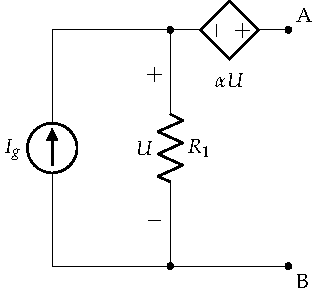
\includegraphics[width=0.7\linewidth]{../figs/Thevenin1.pdf}
    \end{center}
\end{minipage}
\begin{minipage}[c]{0.5\linewidth}
    \textbf{Datos}:
    \vspace{2mm}
    
    $I_g = \qty{10}{\ampere}$\\[5pt]
    $R_1 = \qty{1}{\ohm}$\\[5pt]
    $\alpha = 5$
\end{minipage}


\vspace{3mm}

\hrulefill

\vspace{5mm}
\textbf{Solución}:
\vspace{4mm}

Para calcular $\epsilon_{th}$, es necesario calcular $U_{AB}$ en circuito abierto. 

Aplicando 2LK desde A hasta B, pasando necesariamente por la fuente dependiente de tensión y la resistencia (dado que no conocemos la tensión en el generador de corriente):
\begin{equation*}
  U_{AB} = \alpha U + U = (1 + \alpha) U=(1+5)U=6\,U
\end{equation*}
Además, dado que los terminales A-B están en circuito abierto, toda la corriente del generador $I_g$ circula por la resistencia, luego:
\begin{equation*}
  U = I_g \cdot R_1=10\cdot 1 = \qty{10}{\volt}
\end{equation*}
Por tanto, el generador de Thévenin tiene una \textit{fem} de:
\begin{equation*}
  U_{AB} = 6\, U = 6\cdot 10 = \boxed{\qty{60}{\volt} = \epsilon_{th}}
\end{equation*}

Para calcular la resistencia Thévenin, se apaga la fuente independiente. Como la fuente dependiente permanece, es necesario aplicar un generador de prueba a la salida:

\vspace{3mm}

\begin{minipage}[c]{0.5\linewidth}
    \begin{center}
        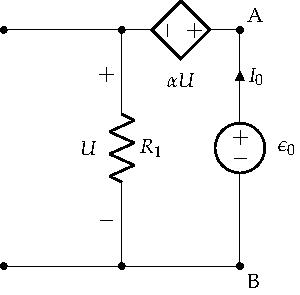
\includegraphics[width=0.7\linewidth]{figs/Thevenin1_fuenteprueba.pdf}
    \end{center}
\end{minipage}
\begin{minipage}[c]{0.5\linewidth}    
    \begin{align*}
      \epsilon_0 &= \alpha U + U = U(1+\alpha) = 6\,U\\[5pt]
      U &= I_0\cdot R_1 = I_0\cdot 1 = I_0
    \end{align*}

    \vspace{3mm}
    Por tanto:

    \begin{equation*}
      R_{th} = \dfrac{\epsilon_0}{I_0}=\dfrac{6\,U}{U} = \boxed{\qty{6}{\ohm}}
    \end{equation*}
\end{minipage}

\end{document}
